\documentclass[10pt]{beamer}
\usepackage{etex}
\newenvironment<>{varblock}[2][\textwidth]{%
  \setlength{\textwidth}{#1}
  \begin{actionenv}#3%
    \def\insertblocktitle{#2}%
    \par%
    \usebeamertemplate{block begin}}
  {\par%
    \usebeamertemplate{block end}%
  \end{actionenv}}
%\usepackage{hyperref}
%\usepackage{natbib}
%\usepackage{beamerthemeshadow}
\usepackage{beamerinnerthemecircles, beamerouterthemeshadow}

% MQ: This is to be able to compile on the Riksbank computer. Uncomment with my laptop. Ugly solution but will have to do for now.
%\usepackage{epstopdf}
%\epstopdfsetup{outdir=./}

\usepackage{amsmath,amssymb,amsfonts}
\usepackage[pdf]{pstricks}
%\usepackage{bbm}
%\usepackage{booktabs}
\usepackage{amsthm}
\usepackage{booktabs}
\usepackage{graphicx}
\usepackage{graphics}
\usepackage{url}
%\usepackage{breqn}
%\usepackage{hyperref}
\usepackage[authoryear]{natbib}
\usepackage{setspace}
\usepackage{multirow}
%\usepackage{harvard}
\usepackage{xcolor}
%\usepackage{multicolumn}
\usepackage{algpseudocode}
\usepackage{sidecap}
\usepackage{bbm} 
\usepackage{courier}
\usepackage{tikz}
\usetikzlibrary{arrows,shapes,snakes,automata,backgrounds,petri}

\tikzset{
  treenode/.style = {align=center, inner sep=0pt, text centered,
    font=\sffamily},
  arn_n/.style = {treenode, circle, white, font=\sffamily\bfseries, draw=black,
    fill=black, text width=1.5em},% arbre rouge noir, noeud noir
  arn_r/.style = {treenode, circle, red, draw=red, 
    text width=1.5em, very thick},% arbre rouge noir, noeud rouge
  arn_x/.style = {treenode, rectangle, draw=black,
    minimum width=0.5em, minimum height=0.5em}% arbre rouge noir, nil
}
\beamertemplatenavigationsymbolsempty

\newenvironment{myenumerate}{\begin{enumerate}[(1)]}{\end{enumerate}} 
\sidecaptionvpos{figure}{c}
% FOR COLORING PARTS  OF TABLE
%\usepackage[beamer,customcolors]{hf-tikz}

%\tikzset{hl/.style={
%    set fill color=red!80!black!40,
%    set border color=red!80!black,
%  },
%}

\mode<presentation> {
    \usetheme{Madrid} %Frankfurt} %Bergen, Berkely, Berlin, Boadilla, CambridgeUS, Darmstadt,
                          %Frankfurt, Goettingen, Singapore, Warsaw
    \usecolortheme{beaver} %seahorse} %default} %beetle, seahorse, wolverine, dolphin, beaver
    %\useoutertheme[subsection=true]{smoothbars} 
    \usefonttheme{default}
    %\usecolortheme{red}
    

	\setbeamercolor{block title}{use=unstructure, fg=white, bg=purple!75!black} %{use=structure,fg=white,bg=purple!75!black}
	%\setbeamercolor{block body}{use=structure,fg=black,bg=white!20!white}    
    %\setbeamercolor{block body}{bg=white}
    \setbeamertemplate{enumerate items}[default]
    \setbeamercolor{enumerate item}{fg=purple!75!black} 
    \setbeamercolor{enumerate subitem}{fg=purple!75!black} 	 
	\setbeamercolor{itemize item}{fg=purple!75!black}  
	\setbeamertemplate{itemize item}[triangle]  
	\setbeamercolor{itemize subitem}{fg=purple!75!black}
	\setbeamertemplate{itemize subitem}[triangle]
	\setbeamertemplate{blocks}[framed]


}



%\usepackage{colortbl}
%\definecolor{yellow}{cmyk}{0,0.18,0.90,0.00}

%\usepackage{xcolor}

%\usepackage[authoryear]{natbib}
\begin{document}
\title[Lecture 1]{Bayesian Learning 732A46: Lecture 1}  
\author[Matias Quiroz]{Matias Quiroz\inst{1}$^{,}$\inst{2}}
\setbeamerfont{institute}{size=\fontsize{7pt}{8pt}}
\institute[LiU and Riksbank]{
  \inst{1}%
   Division of Statistics and Machine Learning, Link\"{o}ping University\\~\\
  \inst{2}%
   Research Division, Sveriges Riksbank\\
     
}

%\institute[Riksbank and LiU]{Sveriges Riksbank and Division of Statistics and Machine Learning, Link\"{o}ping University}

\date[]{March 2016} %\today 

%\usebackgroundtemplate{%
%  \vbox to \paperheight{\vfil\hbox to \paperwidth{\hfil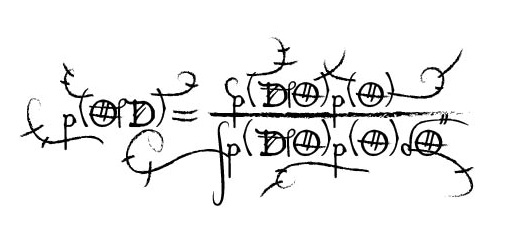
\includegraphics[width=1.5in]{Bayes.jpg}\hfil}\vfil}
%}

{
%\usebackgroundtemplate{\begin{center}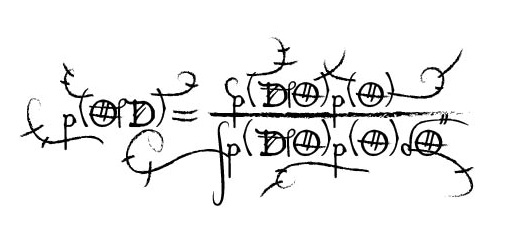
\includegraphics[width=0.4\paperwidth]{Bayes.jpg}\end{center}}
\usebackgroundtemplate{%
  \vbox to \paperheight{\hbox to \paperwidth{\hfil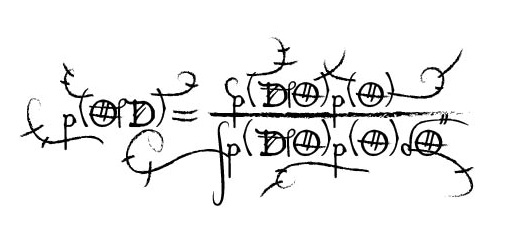
\includegraphics[width=2in]{Bayes.jpg}\hfil}}
}
\begin{frame}
\titlepage
\end{frame}
}
%\frame{\titlepage} 

%\frame{\frametitle{Overview of the talk}\tableofcontents}

\begin{frame}
\frametitle{Course overview}
\begin{itemize}
\item A few words about me
\begin{itemize}
\item {\color{blue}M.Sc. Engineering Mathematics}, Lund University
\item {\color{blue}Ph.D. Statistics}, 2015, Stockholm University 
\\{\color{blue}Supervisor:} \textbf{Mattias Villani}
\item {\color{blue}Doctoral thesis} on \textbf{Markov Chain Monte Carlo} for large data sets.
\item {\color{magenta}I am a Bayesian believer.}
\end{itemize}
\item The course consist of \textbf{12 lectures} and \textbf{4 computer labs}. \\ \textbf{\color{blue}Material}: \href{https://github.com/matiasq/BayesLearningLiU}{https://github.com/matiasq/BayesLearningLiU}

\item Divided into four \textbf{\color{red}modules} (\textbf{3} lectures + \textbf{1} lab each)
\begin{enumerate}
\item The \textbf{basics}, single and multiparameter models.
\item \textbf{Regression} models.
\item Estimating complex models with \textbf{MCMC}.
\item \textbf{Flexible models} and \textbf{Model inference}. 
\end{enumerate}
\item \textbf{\color{blue}Examination}
\begin{itemize}
\item Lab reports (2 credits, work in pairs).
\item An individual project with a written report (4 credits).
\item Oral exam (if needed).
\end{itemize} 
\end{itemize}
\end{frame}

\begin{frame}
\frametitle{Lecture overview}
\begin{itemize}
\item The Bayesian paradigm \bigskip{}

\item The likelihood function \bigskip{}

\item The Bernoulli model \bigskip{}

\item The normal model with known variance
\end{itemize}	
\end{frame}

\begin{frame}
\frametitle{What is a statistical model?}
\begin{itemize}
\item \textbf{Briefly}: A model is a \textbf{\color{red}compact} and \textbf{\color{red}interpretable} representation of the observed data. 
\item \textbf{Elements} of a statistical model
\begin{itemize}
\item \textbf{\color{red}Data} $y=(y_1,\dots,y_n)$.
\item \textbf{\color{red}Parameter(s)} $\theta$.
\item A \textbf{\color{red}probabilistic} model $p(y|\theta)$ - probability theory to represent 
\textbf{\color{blue}the uncertainty} that is inherent in data (noise, natural variation).
\end{itemize}
\item \textbf{Learn} about (\textit{the unknown}) $\theta$. 
\item A statistician deals with \textbf{the uncertainty} regarding $\theta$. True \textbf{\color{blue}regardless if she is a {\color{red}Frequentist} or {\color{red}Bayesian}}!
\item The difference is how she \textbf{thinks about} this uncertainty...


\end{itemize}	
\end{frame}

\begin{frame}
\frametitle{Two different minds...}
\begin{center}
\begin{minipage}{\columnwidth}
\begin{varblock}[0.8\columnwidth]{Reading the mind of a \textbf{\color{yellow}Frequentist} statistician}
I think of $\theta$ as an \textit{unknown} but \textbf{\color{blue}non-random} \textbf{"state of nature"} (fixed quantity). The \textbf{random data} $y$ are generated under this \textbf{fixed} $\theta$ via the model $p(y|\theta)$. I \textbf{could have} obtained \textbf{another dataset}, so I will use \textbf{\color{blue}a repeated sampling argument} to describe my uncertainty about $\theta$.
\end{varblock}
\vspace*{4mm}
\begin{varblock}[0.8\columnwidth]{Reading the mind of a \textbf{\color{yellow}Bayesian} statistician}
There are two quantities present; the data $y$ and the \textbf{"state of nature"} $\theta$. \textbf{\color{blue}I have seen} $y$ but I have \textbf{\color{blue}not seen the unknown} $\theta$. I will therefore regard $\theta$ as random and describe my uncertainty about $\theta$ \textbf{conditional on the data I have seen}.
\end{varblock}

\end{minipage}
\end{center}


\end{frame}


\begin{frame}
\frametitle{The likelihood function}
\begin{itemize}
\item The notation $p(y|\theta)$ for representing the \textbf{probabilistic model} is interpreted in two \textbf{\color{blue}distinct} ways.
\item As a \textbf{\color{red}FUNCTION OF} $y$, for a \textbf{\color{red}FIXED} $\theta$, $p(y|\theta)$ is the \textbf{probability distribution} for the data $y=(y_1, \dots, y_n)$. $\int p(y|\theta)dy=1$
\item As a \textbf{\color{red}FUNCTION OF} $\theta$, for a \textbf{\color{red}FIXED} $y$, $p(y|\theta)$ is the \textbf{likelihood function} for the parameter $\theta$.
\item \textbf{\color{blue}Question}: Is the \textbf{likelihood function} a probability distribution for $\theta$?
\pause
\vspace{3mm}
\begin{figure}[H]

\includegraphics[width=0.25\columnwidth]{nocat}
\end{figure}

\end{itemize}
\end{frame}


\begin{frame}
\frametitle{Inversion of probabilities: Bayes' theorem}
\begin{itemize}
\item Let $H$ and $E$ be two events. 
\item From a basic course in probability: \textbf{\color{blue}Bayes' theorem} relates $\Pr(H|E)$ to $\Pr(E|H)$ $$\Pr(H|E)=\frac{\Pr(E|H)\Pr(H)}{\Pr(E)}, \quad \Pr(E) = \Pr(E|H)\Pr(H) + \Pr(E|H^{c})\Pr(H^{c}).$$
\item For the \textbf{inference problem}
\begin{eqnarray*}
E & = & \text{{\color{red}Evidence}: data } y\\
H & = & \text{{\color{red}Hypothesis} about } \theta \text{ (e.g.: parameter, prediction)}.
\end{eqnarray*}
\item \textbf{\color{blue}Bayes' theorem} for the inference problem (continuous $\theta$)
$$p(\theta|y)=\frac{p(y|\theta)p(\theta)}{p(y)}, \quad p(y)=\int p(y|\theta)p(\theta)d\theta.$$
\item $p(\theta)$ is the \textbf{\color{blue}} prior distribution.
\item $p(\theta|y)$ is a function of $\theta$ with $y$ \textbf{\color{blue}regarded as fixed}.
\item \textbf{\color{blue}Question}: Is $p(\theta|y)$ a probability distribution for $\theta$?
\end{itemize}

\end{frame}



\begin{frame}
\frametitle{The cat is not grumpy anymore!}
\begin{figure}[H]

\includegraphics[width=0.5\columnwidth]{yescat}
%\protect\caption{$\p(\alpha, \beta|y)$}
\end{figure}

\end{frame}

\begin{frame}
\frametitle{Bayesian inference}
\begin{itemize}
\item $p(\theta|y)$ is the \textbf{posterior distribution}. A statement like $$\Pr(\theta \in  [a, b] | y)\quad \text{makes sense. \textbf{\color{blue}Fantastic!}}$$
\begin{center}
\begin{minipage}{\columnwidth}

\begin{center}
\begin{varblock}[0.9\columnwidth]{In a world of classical statistics: {\color{yellow}A difficult question}}
\begin{small}
Let $[a, b]$ be a (classical) confidence interval with significance $\alpha=0.05$. 
\\ \textbf{Conditional on $y$} (i.e. given that we have seen the data), what is the probability that $[a, b]$ covers $\theta$? 
\pause
\\~\\
\textbf{\color{red}Answer:} 0 or 1! \textbf{Why?:} The interval $[a,b]$ is regarded as stochastic w.r.t the data $y$. Once the data is observed, there is no uncertainty anymore. Therefore, a \textbf{frequentist does not condition on the observed data}, but instead \textbf{\color{blue}averages over all possible data} that could have been observed (but were not observed!).
\end{small}
\end{varblock}
\end{center}
\end{minipage}
\end{center}
\item \textbf{Punchline 1:} Bayesian inference is \textbf{\color{blue}conditional} on observed data, whereas classical inference is \textbf{\color{blue}unconditional} (averages over unobserved data).
\item Bayesian inference obeys the \textbf{Likelihood principle}.
\end{itemize}

\end{frame}

\begin{frame}
\frametitle{Bayesian inference, cont.}
\begin{itemize}
\item \textbf{Punchline 2:} Confidence intervals are \textbf{\color{red}hard to interpret} because they are \textbf{\color{red}not probabilities} w.r.t $\theta$. The \textbf{\color{blue}Bayesian posterior} is straightforward.
\item Revisiting the formula
$$p(\theta|y)=\frac{p(y|\theta)p(\theta)}{p(y)}, \quad p(y)=\int p(y|\theta)p(\theta)d\theta.$$
\begin{itemize}
\item \textbf{\color{blue}The prior} $p(\theta)$: your \textbf{subjective belief} about the uncertainty of $\theta$.
\item \textbf{\color{blue}The likelihood} $p(y|\theta)$: the \textbf{information} about $\theta$ contained in $y.$
\item \textbf{\color{blue}The marginal likelihood} $p(y)$: A normalizing constant \textbf{independent} of $\theta$.
\end{itemize}
\item \textbf{Compact form}\begin{eqnarray*}
p(\theta|y) & \propto & p(y|\theta)p(\theta) \\
\mathrm{Posterior} & \propto & \mathrm{Likelihood} \times \mathrm{Prior}.
\end{eqnarray*} 
\end{itemize}

\end{frame}


\begin{frame}
\frametitle{Bayesian inference, cont.}
\begin{itemize}
\item What if $\theta$ is a natural constant? \textbf{Example:} the speed of light. \medskip{}
\item \textbf{Bayesian:} Do you know the value of $\theta$ or not? \medskip{}
\item To a \textbf{Bayesian}, any unknown quantity is a random variable.  \medskip{}
\item \textbf{Subjective probability:} $p(\theta)$ reflects Your knowledge/\textbf{\color{blue}uncertainty} about $\theta$. \medskip{}
\item \textbf{\color{blue}Bayes' theorem:} Updates Your \textbf{subjective prior belief} \textbf{\color{red}objectively} (just maths!) to a \textbf{posterior belief} by combining it with the data via the \textbf{likelihood function}. \medskip{}
\item A probability distribution for $\theta$ is \textbf{useful for decision making}.

\end{itemize}
\end{frame}



\begin{frame}
\frametitle{Bayes in action: Bernoulli model with a Beta prior}
\begin{itemize}
\item \textbf{Model} 
\[
y_{1},...,y_{n}|\theta\overset{iid}{\sim}\mathrm{Bern}(\theta)
\]

\item \textbf{Prior} with \textit{hyper parameters} $\alpha_0$ and $\beta_0$
\[
p(\theta) = \mathrm{Beta}(\theta|\alpha_0,\beta_0) = \frac{\Gamma(\alpha_0+\beta_0)}{\Gamma(\alpha_0)\Gamma(\beta_0)}\theta^{\alpha_0-1}(1-\theta)^{\beta_0-1}\text{ \ for } 0 \leq\theta\leq1.
\]
$\alpha_0$ and $\beta_0$ are \textbf{\color{blue}set by the user to reflect her uncertainty} about $\theta$. 
\item \textbf{Posterior} [$s=\sum_{i=1}^{n}{y_i}$ nbr of successes, $f=n-s$]
\begin{eqnarray*}
p(\theta|y_{1},...,y_{n}) & \propto & p(y_{1},...,y_{n}|\theta)p(\theta)\\
 & \propto & \theta^{s}(1-\theta)^{f}\theta^{\alpha_0-1}(1-\theta)^{\beta_0-1}\\
 & = & \theta^{s+\alpha_0-1}(1-\theta)^{f+\beta_0-1}.
\end{eqnarray*}
\item This is \textbf{\color{red}proportional to} the $\mathrm{Beta}(\theta|\alpha_0+s,\beta_0+f)$ density. 
\item The \textbf{\color{blue}prior-to-posterior} mapping reads
\[
\theta\sim \mathrm{Beta}(\alpha_0,\beta_0)\overset{y_{1},...,y_{n}}{\Longrightarrow}\theta|y_{1},...,y_{n}\sim \mathrm{Beta}(\underbrace{\alpha_0+s}_{\alpha_n},\underbrace{\beta_0+f}_{\beta_n}).
\]

\end{itemize}
\end{frame}


\begin{frame}
\frametitle{Bernoulli model: spam emails}
\begin{itemize}
\item George has gone through his collection of $4601$ e-mails. He classified
$1813$ of them to be spam (and 2788 non-spam).\bigskip{}

\item Let $y_{i}=1$ if $i$th email is spam ($0$ otherwise). Assume $y_{i}|\theta\overset{iid}{\sim} \mathrm{Bern}(\theta)$ and $\theta \sim \mathrm{Beta}(\alpha_0,\beta_0)$ \textbf{\color{blue}a priori}.\bigskip{}

\item \textbf{\color{blue}Posterior}
\[
\theta|y \sim \mathrm{Beta}(\alpha_0+1813, \beta_0+2788).
\]

\end{itemize}

\end{frame}




%% HERE STARTS THE FIGURES OF PRIOR SENSITIVITY
\begin{frame}{Spam data ($n=10$, $s=2$ and $s=8$): prior sensitivity}


\begin{center}
%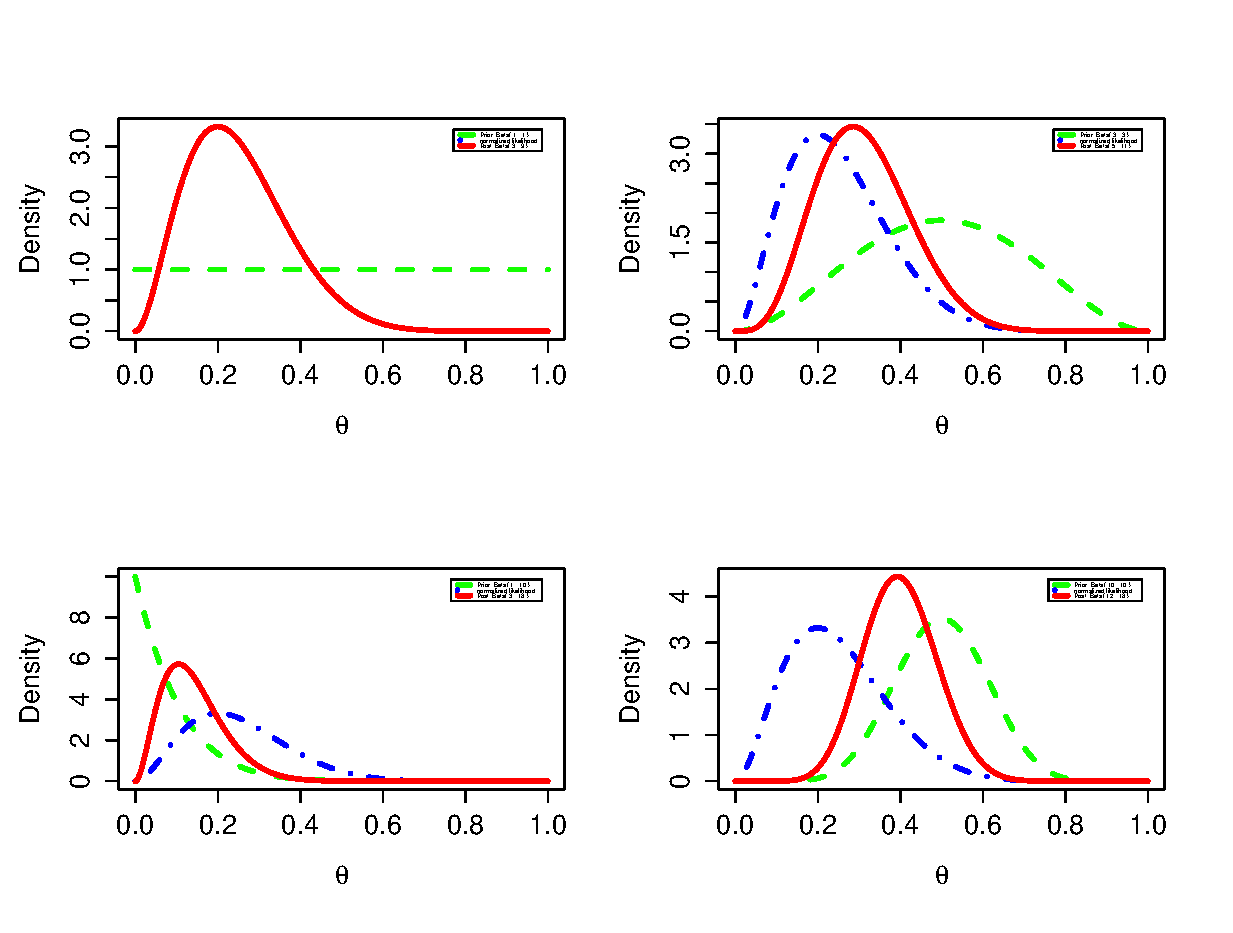
\includegraphics[scale=0.5,bb = 0 0 200 100, draft, type=eps]{SpamDataSmall}
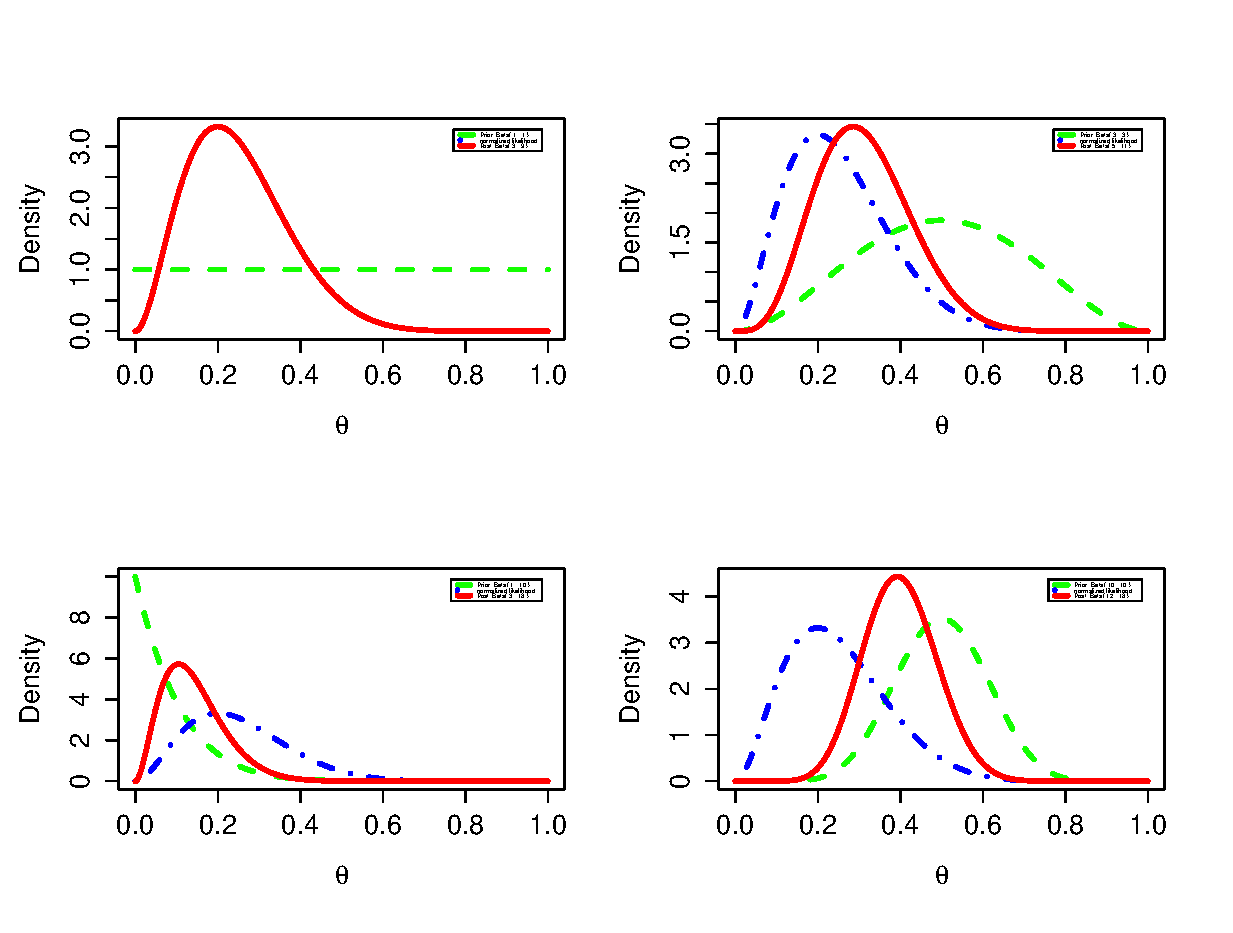
\includegraphics[width=1\columnwidth]{SpamDataSmall}

\par\end{center}

\end{frame}
%
%


\begin{frame}{Spam data ($n=100$, $s=39$ and $s=61$): prior sensitivity}


\begin{center}
%\includegraphics[scale=0.5,bb = 0 0 200 100, draft, type=eps]{/Users/matvi05/Dropbox/Projects/BayesBook/Figures/SpamDataMedium.eps}
\includegraphics[width=1\columnwidth]{SpamDataMedium}

\par\end{center}

\end{frame}

\begin{frame}{Spam data ($n=4601$, $s=1813$ and $s=2788$): prior sensitivity}


\begin{center}
%\includegraphics[scale=0.5,bb = 0 0 200 100, draft, type=eps]{/Users/matvi05/Dropbox/Projects/BayesBook/Figures/SpamDataFull.eps}
\includegraphics[width=0.9\columnwidth]{SpamDataFull}

\par\end{center}

\end{frame}

\begin{frame}{Spam data: Posterior convergence}


\begin{center}
%\includegraphics[scale=0.5,bb = 0 0 200 100, draft, type=eps]{/Users/matvi05/Dropbox/Teaching/StatMetoder2010/F2/eps/spamConvergencePosterior.eps}
\includegraphics[width=0.8\columnwidth]{spamConvergencePosterior}

\par\end{center}


\end{frame}


%% HERE ENDS THE FIGURES OF PRIOR SENSITIVITY



\begin{frame}
\frametitle{Normal model with known variance and a uniform prior}
\begin{itemize}
\item \textbf{Model} 
\[
y_{1},...,y_{n}|\theta\overset{iid}{\sim}\mathcal{N}(\theta, \sigma^2), \quad [\sigma^2 \text{ is} \textbf{ \color{red} known}.]
\]

\item \textbf{Prior} 
\[
p(\theta) \propto c\text{ (a constant)}.
\]
 
\item \textbf{Likelihood} [\textbf{\color{blue}white board!}]
\begin{eqnarray*}
p(y_{1},...,y_{n}|\theta) & = & \prod_{i=1}^{n}(2\pi\sigma^{2})^{-1/2}\exp\left[-\frac{1}{2\sigma^{2}}(y_{i}-\theta)^{2}\right]\\
 & \propto & \exp\left[-\frac{1}{2(\sigma^{2}/n)}(\theta-\bar{y})^{2}\right].
\end{eqnarray*}

\item \textbf{Posterior}
\[
\theta|y_{1},...,y_{n}\sim \mathcal{N}(\underbrace{\bar{y}}_{\mu_n},\underbrace{\sigma^{2}/n}_{\tau^2_n})
\]

\item \textbf{\color{blue}Make your life easy}: \textbf{throw away} normalizing constants independent of $\theta$!
\end{itemize}
\end{frame}



\begin{frame}
\frametitle{Some remarks}
\begin{itemize}
\item \textbf{The prior} $p(\theta) \propto c$ is \textbf{\color{red}improper}: $\int p(\theta) d\theta = \infty$.
\item \textbf{\color{red}WARNING:} \textbf{improper priors} may lead to \textbf{improper posteriors}. \textbf{Not valid} since the posterior is (by construction) a probability distribution $$\int p(\theta|y) d\theta = 1.$$ 
\item This prior is said to be \textbf{\color{blue}non-informative} because it \textbf{does not favor} any $\theta$ a priori. More on this later.
\item The \textbf{posterior mode} is $\mu_n = \bar{y}$. Coincides with the \textbf{maximum likelihood estimator} $$\mu_{\mathrm{MLE}}=\bar{y}.$$
\item We will learn that \textbf{Bayesian inference with a non-informative prior} gives the same \textbf{point estimates} as classical inference...
\item ... but a \textbf{different interpretation} $$\text{Posterior = a probability distribution = \textbf{\color{blue}fun inference!}}$$

\end{itemize}
\end{frame}




\begin{frame}{Prior information in the Normal model - the normal prior}


\begin{itemize}
\item \textbf{Prior} 
\[
\theta \sim \mathcal{N}(\mu_{0},\tau_{0}^{2}).
\]

\item \textbf{Posterior}
\begin{eqnarray*}
p(\theta|y_{1},...,y_{n}) & \propto & p(y_{1},...,y_{n}|\theta)p(\theta)\\
 & \propto & \mathcal{N}(\theta|\mu_{n},\tau_{n}^{2}),
\end{eqnarray*}
where
\[
\frac{1}{\tau_{n}^{2}}=\frac{n}{\sigma^{2}}+\frac{1}{\tau_{0}^{2}} \quad \textbf{and}\quad \mu_{n}=w\bar{y}+(1-w)\mu_{0}
\]
with
\[
w=\frac{\frac{n}{\sigma^{2}}}{\frac{n}{\sigma^{2}}+\frac{1}{\tau_{0}^{2}}}.
\]
\item \textbf{\color{blue}White board}: \textbf{tedious} but a good exercise. \textbf{Hint:} the joy of ignoring a constant.
\item \textbf{\color{blue}Interpretation} of the posterior as a \textbf{\color{red}combination of prior and data information}.
\end{itemize}


\end{frame}


\begin{frame}{A combination of prior and data information}
\begin{itemize}
\item Define the \textbf{\color{blue}precision} as the \textbf{reciprocal} of the variance
$$\mathrm{Precision} = \mathrm{Variance}^{-1} = \frac{1}{\mathrm{Variance}}$$
\item Thus
$$\mathrm{Prior~Precision} = \frac{1}{\tau_0^2}, \quad \mathrm{Data~Precision} = \left(\frac{\sigma^2}{n}\right)^{-1} = \frac{n}{\sigma^2}$$
\item Reading the equations \textbf{out loud} (for the normal model with normal prior)
\begin{eqnarray*}
{\color{red}\mathrm{Posterior~Precision}} & = & \mathrm{Data~Precision} + \mathrm{Prior~Precision} \\
{\color{red}\mathrm{Posterior~mean}} & = & \underbrace{\frac{\mathrm{Data~Precision}}{\mathrm{Posterior~Precision}}}_{w}\times (\mathrm{Data~mean}) \\
& + &  \underbrace{\frac{\mathrm{Prior~Precision}}{\mathrm{Posterior~Precision}}}_{1-w}\times(\mathrm{Prior~mean}).
\end{eqnarray*}


\end{itemize}
\end{frame}


\begin{frame}{Some remarks}
\begin{itemize}
\item Note that, informally, if $\tau_0^2 = \infty$ then $\mathrm{Prior~Precision}=0$ and 
\begin{eqnarray*}
{\color{red}\mathrm{Posterior~mean}} & = & \mathrm{Data~mean}
\end{eqnarray*}
\item The \textbf{improper prior} $p(\theta) \propto c$ is the limit $$p(\theta)=\mathcal{N}(\mu_0, \tau_0^2), \quad \text{when }  \tau^2_0 \rightarrow \infty.$$
\item \textbf{\color{blue}My two cents}: I never use "non-informative" priors. I choose a proper prior with hyper parameters that allow \textbf{for a wide range} of $\theta$ values instead...
\item ... but\textbf{ only if I lack prior} information. Otherwise I incorporate prior information.
\item \textbf{\color{red}Don't be ashame} of using priors.
\begin{itemize}
\item It is \textbf{\color{blue}a part of your model}. 
\item Is someone \textbf{accusing you} for a subjective analysis? \textbf{\color{blue}My two cents}: nothing in a model is more subjective than the model itself.
\item It \textbf{makes sense to include prior information}. E.g. if doing a study on a drug, previous experiments are interesting.
\item Prior information is \textbf{often implicitly used in classical statistics}. But it is hidden!
\end{itemize}
\end{itemize}
\end{frame}



\end{document}

